\documentclass[11pt,fleqn,twoside]{article}
\usepackage{makeidx}
\makeindex
\usepackage{palatino} %or {times} etc
\usepackage{plain} %bibliography style 
\usepackage{amsmath} %math fonts - just in case
\usepackage{amsfonts} %math fonts
\usepackage{amssymb} %math fonts
\usepackage{lastpage} %for footer page numbers
\usepackage{fancyhdr} %header and footer package
\usepackage{mmpv2} 
\usepackage{url}
\usepackage{float}
\usepackage{longtable}
\usepackage{pdfpages}

% the following packages are used for citations - You only need to include one. 
%
% Use the cite package if you are using the numeric style (e.g. IEEEannot). 
% Use the natbib package if you are using the author-date style (e.g. authordate2annot). 
% Only use one of these and comment out the other one. 
\usepackage{cite}
\usepackage[parfill]{parskip}
%\usepackage{natbib}

\begin{document}

\name{Aidan Wynne Fewster}
\userid{awf1}
\projecttitle{NHS Wales Injectable Medicines Guide}
\projecttitlememoir{NHS Wales Android application} %same as the project title or abridged version for page header
\reporttitle{Test Results}
\version{1.0}
\docstatus{Release}
\modulecode{CS39440}
\degreeschemecode{G400}
\degreeschemename{Computer Science}
\supervisor{Andrew Starr} % e.g. Neil Taylor
\supervisorid{aos}
\wordcount{}

%optional - comment out next line to use current date for the document
\documentdate{20th April 2014} 
\mmp

\setcounter{tocdepth}{3} %set required number of level in table of contents

This document will provide the result for any testing that was carried out on the application. It will include the results of the unit tests, the results of the intergration tests and the results of stress testing the application.


%==============================================================================
\section{Intergration Tests}
%==============================================================================
 To test that the application works as expected a list of integration tests were made and then ran on two devices, one device running API version 19 and the other running API version 8 Using two devices, with varying ages increases the accuracy of the results. To further increase the accuracy of the results the tests would be executed on more devices. 
\begin{center}
\begin{longtable}{| p{5cm} | p{5cm} | c | c |}

\hline
\textbf{Test}                                                              & \textbf{Expected result}                                                                         & \textbf{API 8 result} & \textbf{API 19 result} \\ \hline
\textbf{Login Activity}                                                    & \textbf{}                                                                                        &                       &                        \\ \hline
Enters invalid password and attempt to login                               & User is notified via toast that username is incorrect                                            & \textbf{PASS}         & \textbf{PASS}          \\ \hline
Attempt to login whilst in flight mode                                     & User is notified of connection error                                                             & \textbf{PASS}         & \textbf{PASS}          \\ \hline
Attempt to login using correct details                                     & Download activity is launched                                                                    & \textbf{PASS}         & \textbf{PASS}          \\ \hline
                                                                           &                                                                                                  & \textbf{PASS}         & \textbf{PASS}          \\ \hline
\textbf{Download activity}                                                 &                                                                                                  & \textbf{PASS}         & \textbf{PASS}          \\ \hline
User presses back button                                                   & Return to login screen                                                                           & \textbf{PASS}         & \textbf{PASS}          \\ \hline
User minimises application and re-enters                                   & Download continues in background                                                                 & \textbf{PASS}         & \textbf{PASS}          \\ \hline
Calculator download fails                                                  & Dialog asking the user whether they would like to retry is displayed                             & \textbf{PASS}         & \textbf{PASS}          \\ \hline
Index download fails                                                       & Dialog asking the user whether they would like to retry is displayed                             & \textbf{PASS}         & \textbf{PASS}          \\ \hline
Drug information download fails                                            & Dialog asking the user whether they would like to retry is displayed                             & \textbf{PASS}         & \textbf{PASS}          \\ \hline
User clicks the retry button                                               & The appropriate download task is restarted                                                       & \textbf{PASS}         & \textbf{PASS}          \\ \hline
User clicks cancel button                                                  & User is logged out and login activity is displayed                                               & \textbf{PASS}         & \textbf{PASS}          \\ \hline
                                                                           &                                                                                                  & \textbf{}             & \textbf{}              \\ \hline
\textbf{Main activity}                                                     &                                                                                                  & \textbf{}             & \textbf{}              \\ \hline
User presses back button                                                   & Close application                                                                                & \textbf{PASS}         & \textbf{PASS}          \\ \hline
Check last update date is set correctly                                    & The date within the last updated TextView contains the date the database was last updated        & \textbf{PASS}         & \textbf{PASS}          \\ \hline
Browse drugs button press                                                  & Open the browser drugs activity                                                                  & \textbf{PASS}         & \textbf{PASS}          \\ \hline
Browse calculator button presses                                           & Open the browser calculator activity                                                             & \textbf{PASS}         & \textbf{PASS}          \\ \hline
Update button pressed                                                      & Open the download activity                                                                       & \textbf{PASS}         & \textbf{PASS}          \\ \hline
                                                                           &                                                                                                  & \textbf{}             & \textbf{}              \\ \hline
\textbf{Browse drugs}                                                      &                                                                                                  & \textbf{}             & \textbf{}              \\ \hline
Drugs are displayed properly                                               & Full list of available drugs are displayed within the list                                       & \textbf{PASS}         & \textbf{PASS}          \\ \hline
User enters text into the search box                                       & The lists of drugs are filtered by the inputted text                                             & \textbf{PASS}         & \textbf{PASS}          \\ \hline
User clicks drug                                                           & View drug activity is launched for that drug                                                     & \textbf{PASS}         & \textbf{PASS}          \\ \hline
                                                                           &                                                                                                  & \textbf{}             & \textbf{}              \\ \hline
\textbf{Browse calculators}                                                &                                                                                                  & \textbf{}             & \textbf{}              \\ \hline
Drugs are displayed properly                                               & Full list of drugs with calculators are displayed within the list                                & \textbf{PASS}         & \textbf{PASS}          \\ \hline
User enters text into the search box                                       & The lists of drugs are filtered by the inputted text                                             & \textbf{PASS}         & \textbf{PASS}          \\ \hline
User clicks drug                                                           & Calculator is launched for that drug                                                             & \textbf{PASS}         & \textbf{PASS}          \\ \hline
                                                                           &                                                                                                  & \textbf{}             & \textbf{}              \\ \hline
\textbf{View drug activity}                                                &                                                                                                  & \textbf{}             & \textbf{}              \\ \hline
The correct drug is displayed                                              & The drug selected by the user is displayed                                                       & \textbf{PASS}         & \textbf{PASS}          \\ \hline
User clicks on header helper button                                        & The helping information for the header is displayed.                                             & \textbf{PASS}         & \textbf{PASS}          \\ \hline
User clicks calculator button                                              & The calculator activity is opened                                                                & \textbf{PASS}         & \textbf{PASS}          \\ \hline
                                                                           &                                                                                                  & \textbf{}             & \textbf{}              \\ \hline
\textbf{Calculator test}                                                   &                                                                                                  & \textbf{}             & \textbf{}              \\ \hline
A dosage calculation using correct values is performed by the user         & The results of the calculation and an explanation for the equation used is displayed to the user & \textbf{PASS}         & \textbf{PASS}          \\ \hline
An infusion rate calculation using correct values is performed by the user & The results of the calculation and an explanation for the equation used is displayed to the user & \textbf{PASS}         & \textbf{PASS}          \\ \hline
User enter 0kg for weight                                                  & Error about weight is displayed to user                                                          & \textbf{PASS}         & \textbf{PASS}          \\ \hline
User leaves weight field empty                                             & Error about weight is displayed to user                                                          & \textbf{PASS}         & \textbf{PASS}          \\ \hline
User enters weight of 5kg                                                  & A warning is displayed to the user regarding the weight                                          & \textbf{PASS}         & \textbf{PASS}          \\ \hline
User enters weight of 500kg                                                & A warning is displayed to the user regarding the weight                                          & \textbf{PASS}         & \textbf{PASS}          \\ \hline
User enters 0 for dosage                                                   & Error about dosage is displayed to user                                                          & \textbf{PASS}         & \textbf{PASS}          \\ \hline
User leaves dosage field empty                                             & Error about dosage is displayed to user                                                          & \textbf{PASS}         & \textbf{PASS}          \\ \hline
User enters 0 for time                                                     & Error about time is displayed to user                                                            & \textbf{PASS}         & \textbf{PASS}          \\ \hline
User leaves time field empty                                               & Error about time is displayed to user                                                            & \textbf{PASS}         & \textbf{PASS}          \\ \hline
User enters 0 for concentration                                            & Error about concentration is displayed to user                                                   & \textbf{PASS}         & \textbf{PASS}          \\ \hline
User leaves concentration field empty                                      & Error about concentration is displayed to user                                                   & \textbf{PASS}         & \textbf{PASS}          \\ \hline
                                                                           &                                                                                                  & \textbf{}             & \textbf{}              \\ \hline
\textbf{Common}                                                            &                                                                                                  & \textbf{}             & \textbf{}              \\ \hline
Exit menu item pressed                                                     & Application is terminated                                                                        & \textbf{PASS}         & \textbf{PASS}          \\ \hline
Logout menu item pressed                                                   & User is logged out and then the login activity is opened                                         & \textbf{PASS}         & \textbf{PASS}          \\ \hline
Home menu item pressed                                                     & The main activity is launched                                                                    & \textbf{PASS}         & \textbf{PASS}          \\ \hline
Update item pressed                                                        & The download activity is launched                                                                & \textbf{PASS}         & \textbf{PASS}          \\ \hline
Update item pressed                                                        & The download activity is launched                                                                & \textbf{PASS}         & \textbf{PASS}          \\ \hline
Browse drugs item pressed                                                  & The browse drugs activity is launched                                                            & \textbf{PASS}         & \textbf{PASS}          \\ \hline
Browse calculator pressed                                                  & The browser calcualtor activity is launched                                                      & \textbf{PASS}         & \textbf{PASS}          \\ \hline
\end{longtable}
\end{center}

%==============================================================================
\section{JUnit test results}
%==============================================================================
Unit tests were written for every class of the application, testing each public and protected method. Most tests contained multiple assertions, testing that the expected output was returned when correct information is entered and that an error is raised when the incorrect data is entered.

The following pages contain the results of the Unit tests.

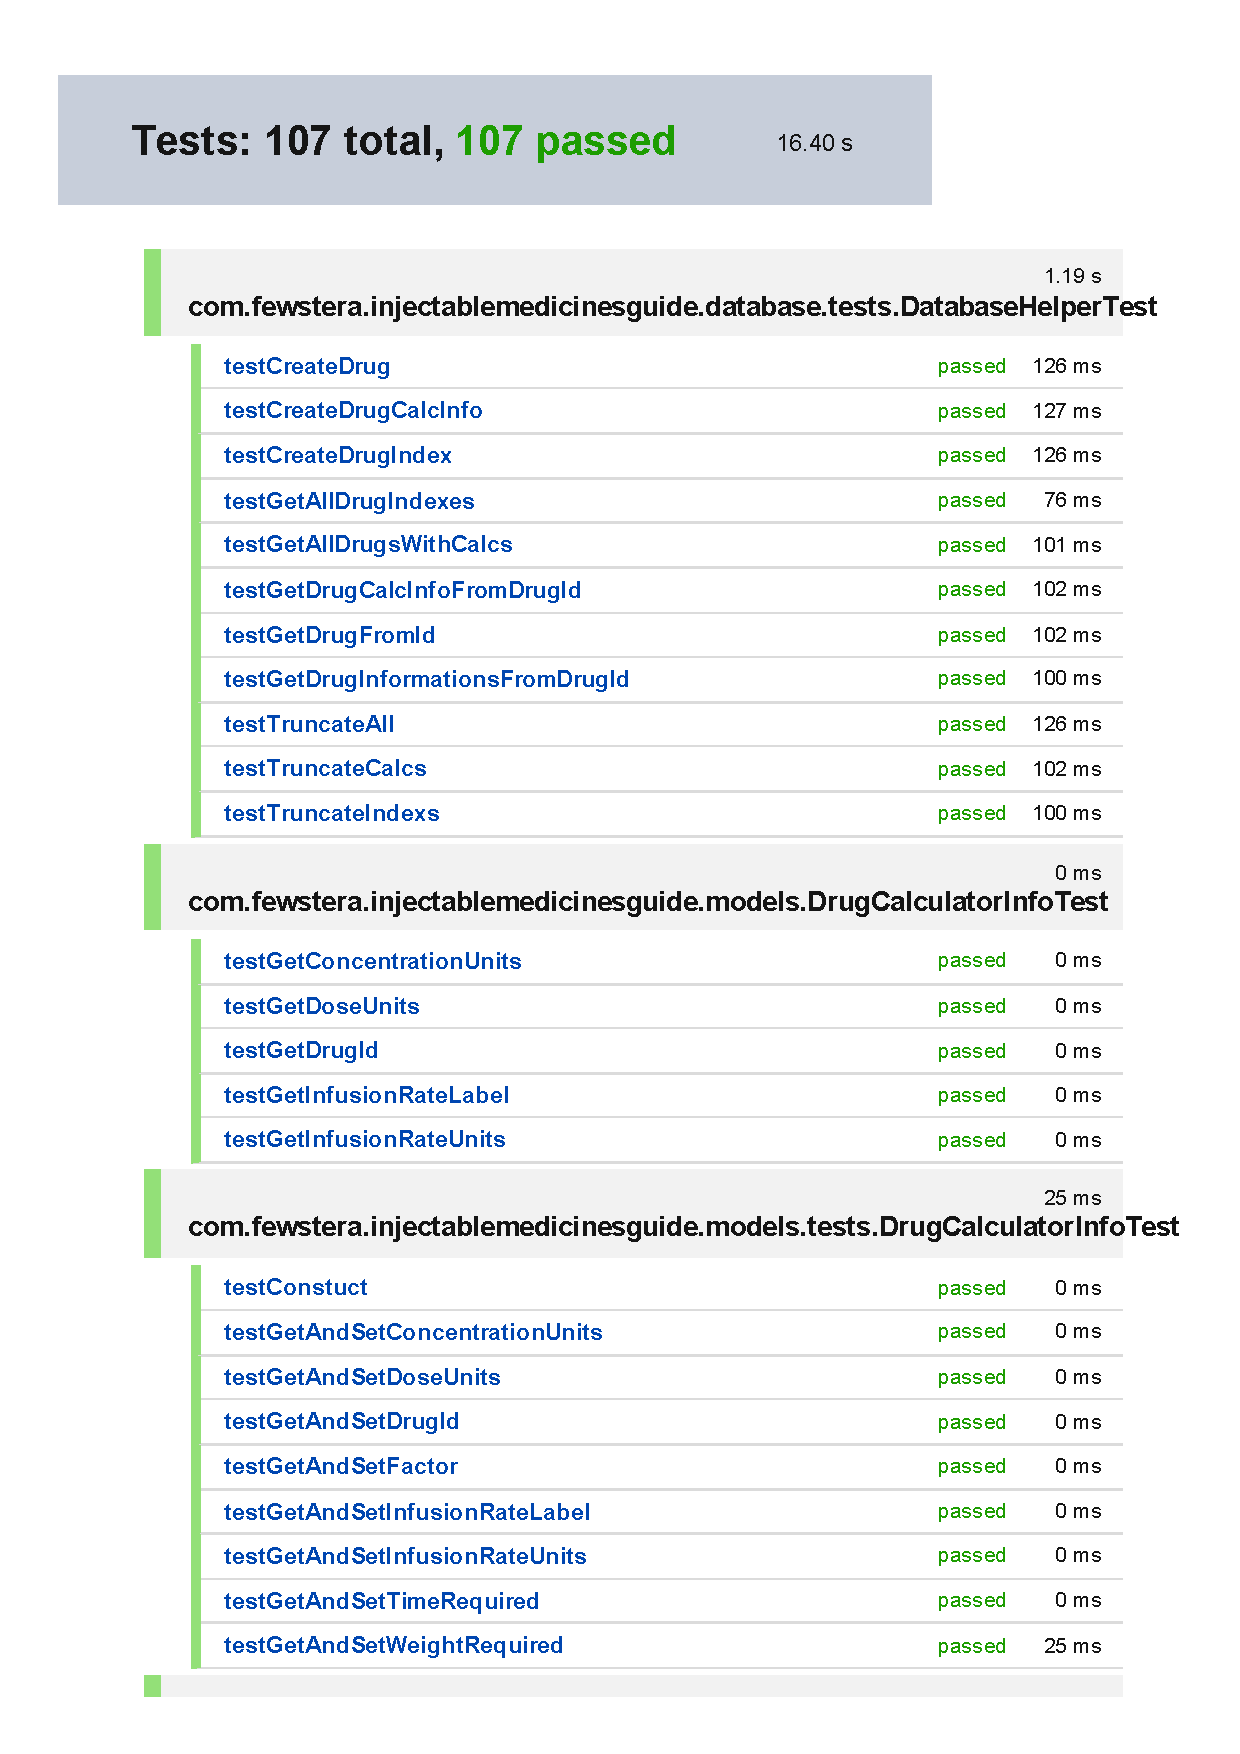
\includepdf[pages=-]{docs/unitTests.pdf} 

%==============================================================================
\section{Exerciser monkey stress text}
%==============================================================================
Exerciser Monkey is a tool provided with the Android SDK, which is used for stress testing Android applications. The tool simulates a set amount of random events on the device, such as button presses, screen presses, volume changes and screen rotations. The tests are used to ensure that applications run well under stressful tasks and that parts of the application do not throw errors.

It was planned that the application would be installed on a device, then using Exerciser Monkey, execute 5000 random events to the device.

Below is the result of executing 5000 random events to the device.

\begin{verbatim}
$ adb shell monkey -p com.fewstera.injectablemedicinesguide 5000
    // activityResuming(com.fewstera.injectablemedicinesguide)
    // activityResuming(com.fewstera.injectablemedicinesguide)
    // activityResuming(com.fewstera.injectablemedicinesguide)
    // activityResuming(com.fewstera.injectablemedicinesguide)
    // activityResuming(com.fewstera.injectablemedicinesguide)
    // activityResuming(com.android.launcher)
    // activityResuming(com.android.launcher)
    // activityResuming(com.android.launcher)
    // activityResuming(com.android.launcher)
    // activityResuming(com.android.launcher)
Events injected: 5000
## Network stats: elapsed time=11069ms (0ms mobile, 11065ms wifi, 4ms not connected)
\end{verbatim}

The tests results show that the test was successful as no time-out warnings, exceptions or errors were thrown by the debugging console.

\end{document}
